%%
%%  Department of Electrical, Electronic and Computer Engineering.
%%  EPR400/2 Project Proposal - Section 3.
%%  Copyright (C) 2011-2017 University of Pretoria.
%%

\section{Project plan}

This section includes the planning for the complete project period which spans over the period 1 February 2017 to 30 November 2017. The planning is in the form of a Gantt chart with a one week resolution. Figure \ref{fig:Gantt1} below shows the planning for the project up to the date of handing in this report. The blocks coloured in blue therefore represent work that is already completed.\\

\begin{figure}[htbp]
    \centering
        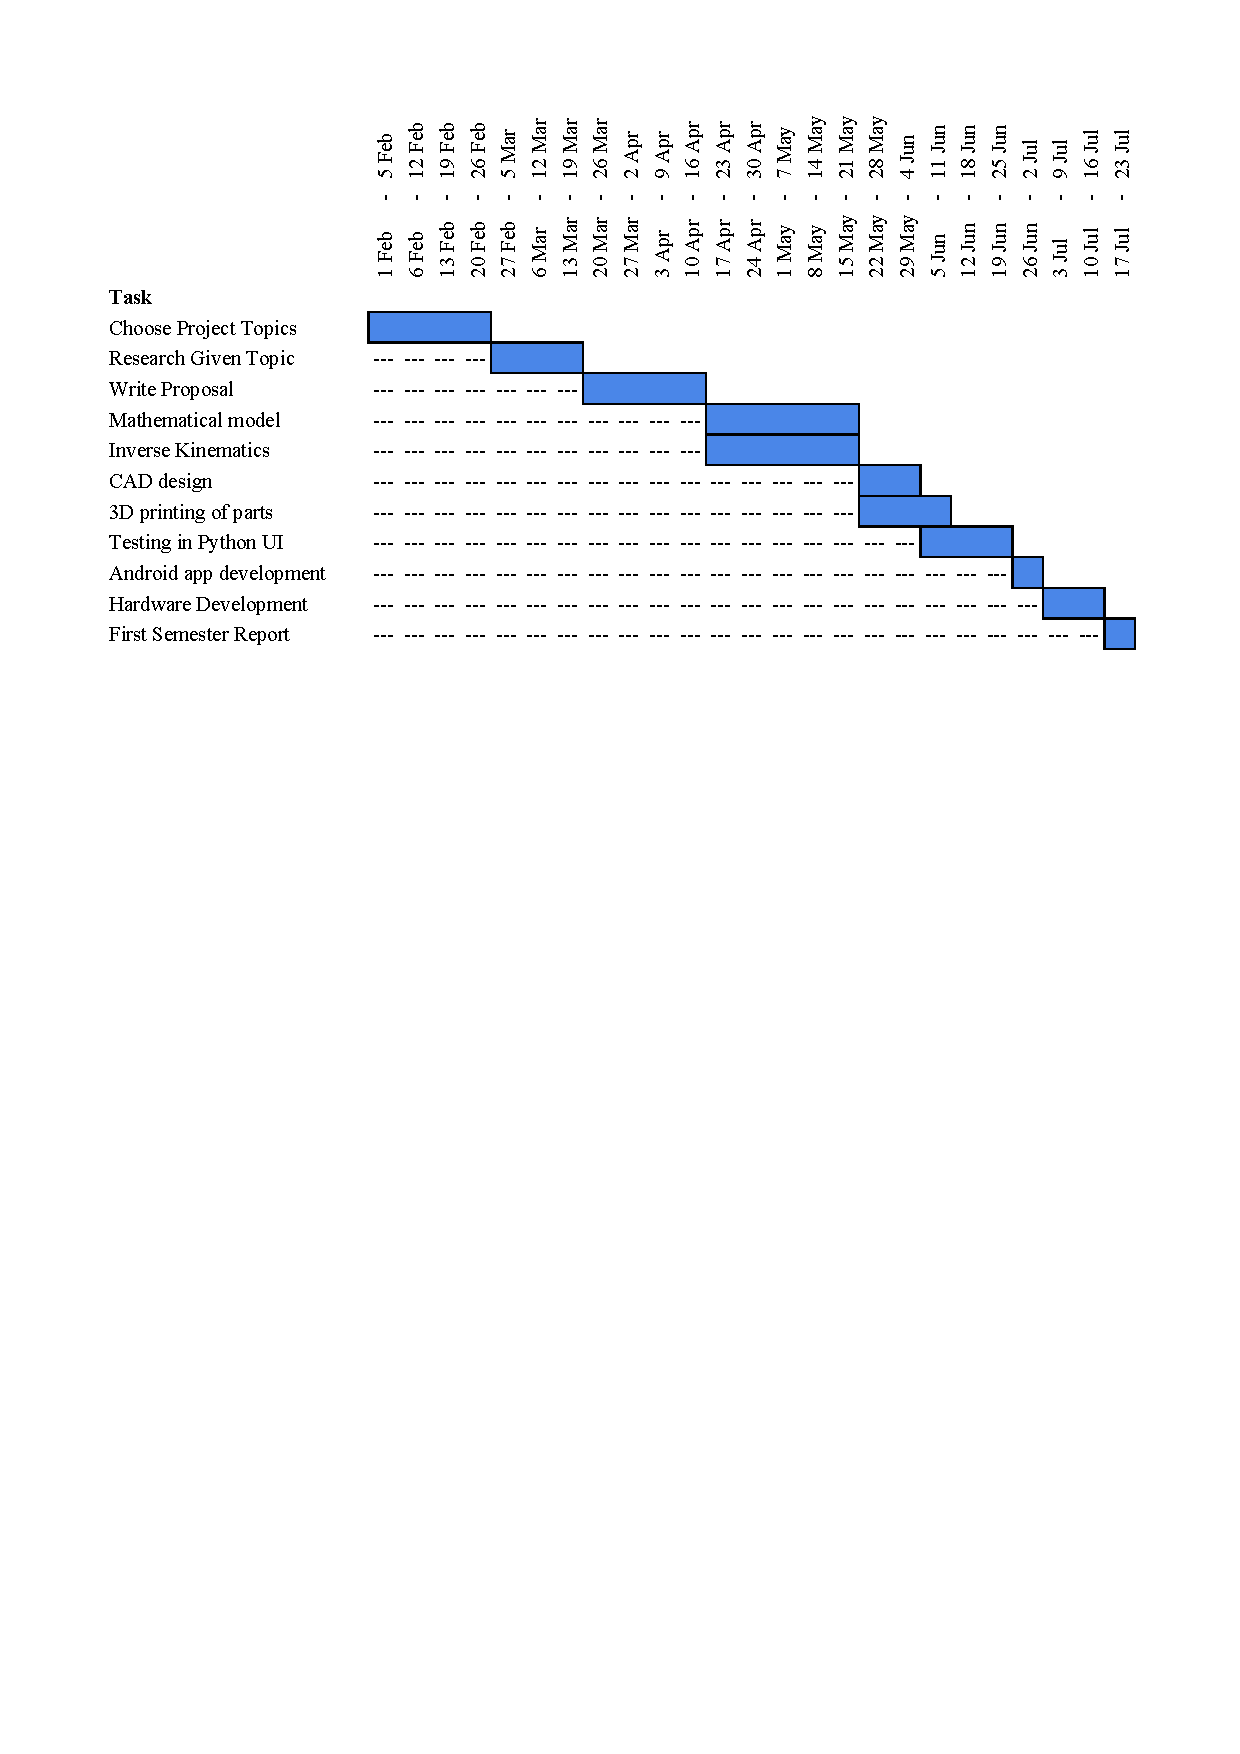
\includegraphics[clip, trim=1.5cm 18cm 1.5cm 1.5cm, width=1.00\textwidth]{pics/Gantt1.pdf}
    \caption{Gantt diagram for work already completed}
    \label{fig:Gantt1}
\end{figure}

Figure \ref{fig:Gantt2} below shows the remaining time in the project period. The blocks coloured in purple therefore represent work that still has to be completed.

\FloatBarrier
\begin{figure}[H]
    \centering
        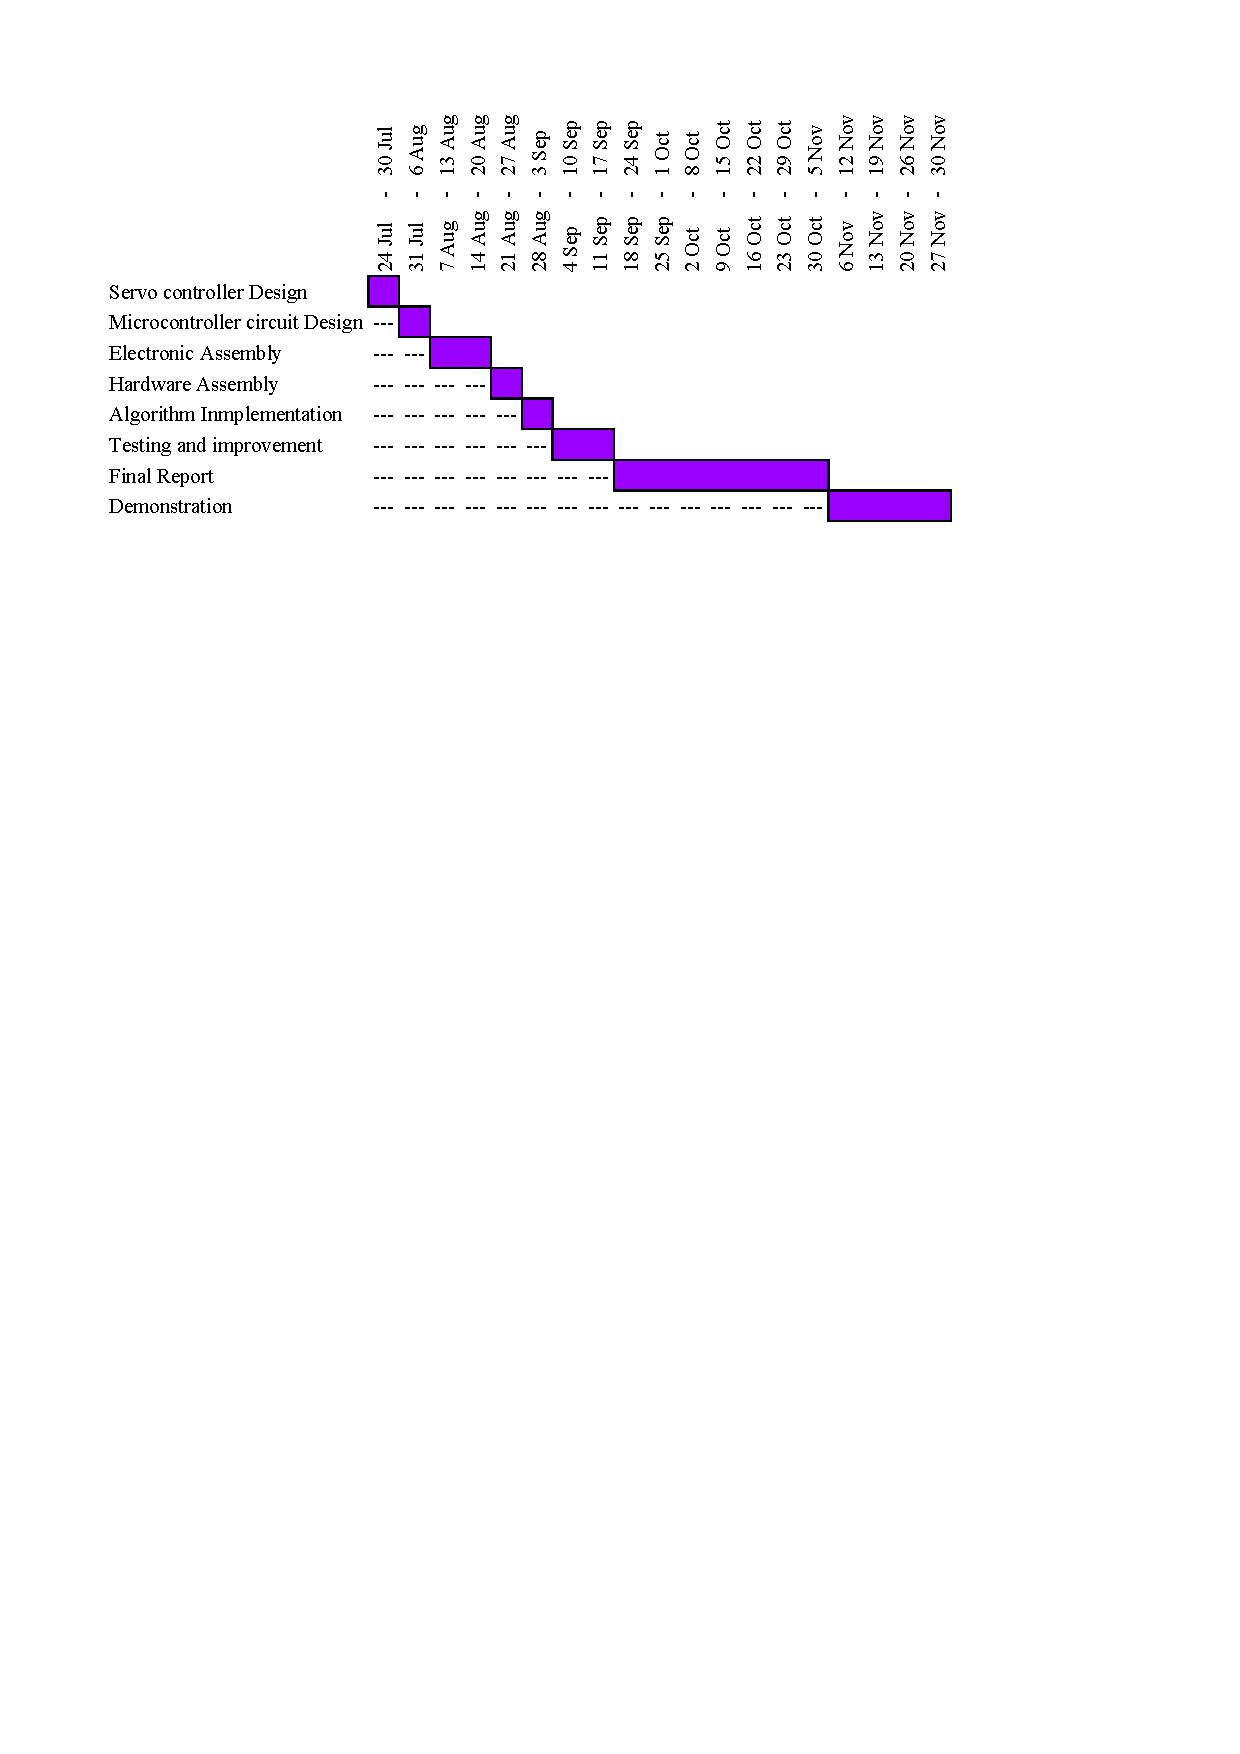
\includegraphics[clip, trim=1.5cm 21cm 1.5cm 1.5cm, width=1.00\textwidth]{pics/Gantt2.pdf}
    \caption{Gantt diagram for work to be completed}
    \label{fig:Gantt2}
\end{figure}
\FloatBarrier

%\vspace{30cm}

%\newpage

%% End of File.

